\documentclass[a4paper]{article}

%% Language and font encodings
\usepackage[english]{babel}
\usepackage[utf8x]{inputenc}
\usepackage[T1]{fontenc}

%% Sets page size and margins
\usepackage[a4paper,top=3cm,bottom=2cm,left=3cm,right=3cm,marginparwidth=1.75cm]{geometry}

%% Useful packages
\usepackage{amsmath}
\usepackage{amssymb}
\usepackage{graphicx}
\usepackage{float}
\usepackage[colorinlistoftodos]{todonotes}
\usepackage[colorlinks=true, allcolors=blue]{hyperref}
\usepackage{listings}
\usepackage[numbered]{matlab-prettifier}
\usepackage{algorithm}
\usepackage{algpseudocode}

\graphicspath{{./figures/}}
\lstMakeShortInline[style=Matlab-editor]"

\title{Handin 2 }
\author{Magnus Wallgren tfy13mwa\\ Wilhelm Lundström fte13wlu}

\begin{document}
\maketitle
\section*{Exercise 1}
Please, see attached matlab code.
\section*{Exercise 2}

Solving the traveling salesman problem for the matrix in exercise 3 we get the optimal path $$x = \{1, 4, 9, 5, 2, 8, 3, 7, 6\}. $$
The total path cost is 
$$f_{\text{opt}} = 1580.$$

\section*{Exercise 3}
In this exercise we construct a number of cities with a distance matrix $D$ where $D_{ij}$ is the cost to travel from city $i$ to city $j$. The matrix is randomly generated with the following constraints:
$$D_{ij} = D_{ji} \quad D_{ii} = 0 \quad D_{i,j} \geq D_{i-1,j} - D_{i-1,j-1}$$

Then we timed how long it took to solve the traveling salesman problem for the matrix $D$ for matrix sizes 2 to 13. Figure \ref{fig:time} shows 95 \% confidence intervals for the time for matrix sizes 2 to 11. The estimated mean run time increases with larger matrix sizes but so does the variance. It is therefore difficult to determine the relation between matrix size and execution time, other than that it increases fast. 

\begin{figure}[H]
\centering
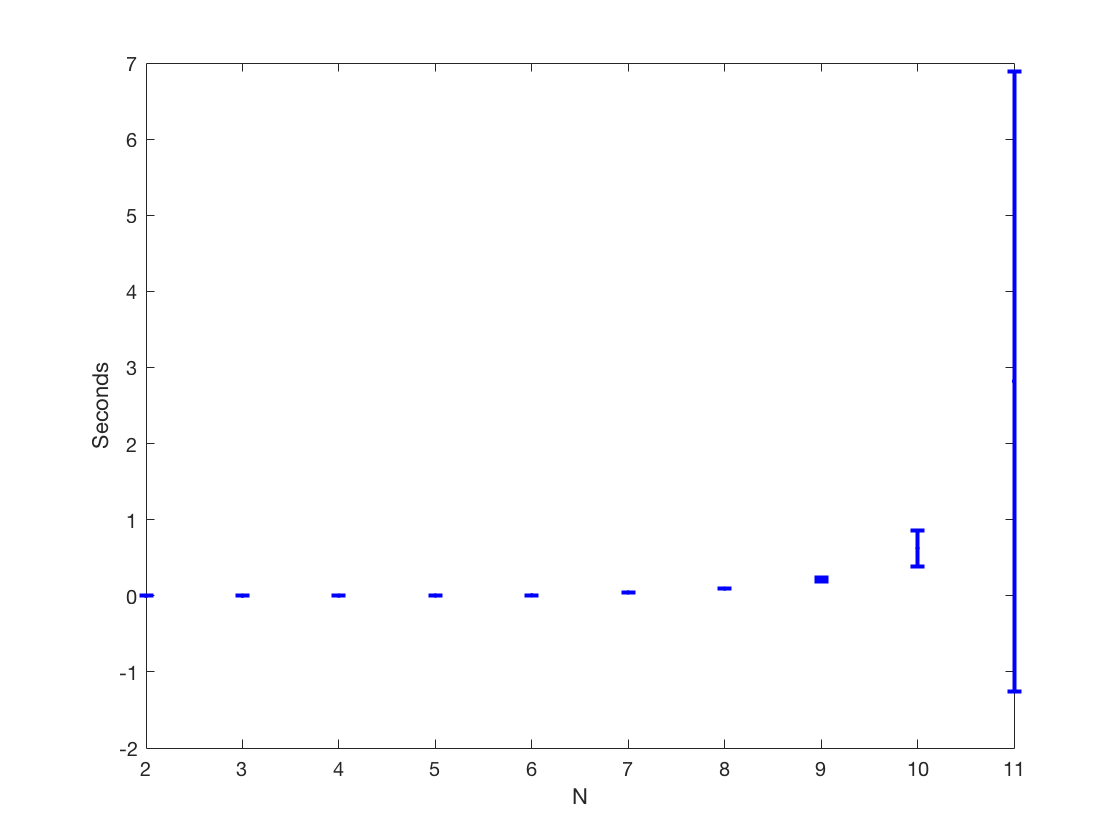
\includegraphics[width=0.6\textwidth]{time}
\caption{This figure shows 95 \% confidence intervals for run times using different number of cities.}
\label{fig:time}
\end{figure}

\end{document}